\chapter{Nonlinear Systems of Differential Equations}
The world is non-linear!  Well shoot. It might seem that this means that for {\it real}
problems we can't use anything that we've done so far.   Wrong!  There are plenty of
things that we can do with nonlinear problems.  For the most part we will rely on a basic
premise from Calculus: up close, a nonlinear function looks linear. You did this back in
calculus when you found tangent lines and tangent planes but now we're going to do the
same for matrices and nonlinear differential equations.  For most of the problems in this
chapter it will be helpful to have MATLAB up so you can plot phase planes and analyze
equilibria graphically.

\section{Modeling a Nonlinear System}
% \begin{problem}
%     We're going to try a social experiment.  
%     \begin{enumerate}
%         \item[(a)] Everyone in the class get a random number between 1 and 5. 
%         \item[(b)] I'm sorry, but if your random number is ``1'' then you just got infected
%             with the horribly contagious disease ODEbola.  Raise your hand if you are
%             infected.
%         \item[(c)] For the next 15 seconds everyone needs to walk aimlessly around the
%             classroom (move the tables out of the way and don't be afraid to bump into
%             each other).  This step is supposed to simulate {\it homogeneous mixing} so
%             \ldots mix homogeneously!
%         \item[(d)] At the end of the 15 seconds stop and stand still.  Reach your arms
%             out.  If someone within arm's reach is infected with ODEbola then you now are
%             too!  Raise your hand if you are infected.
%         \item[(e)] Repeat steps (c) and (d) again. At the end of every step 10\% of the
%             infected people that are infected will recover and are removed from the
%             experiment.  Keep track of the number of
%             people that are infected and recovered at each step.  Run the experiment for
%             several iterations
%     \end{enumerate}
% \end{problem}

\begin{problem}\label{prob:SIR_outbreak_simulation}
    Watch the video \href{https://youtu.be/NSNWDUXN2p4}{https://youtu.be/NSNWDUXN2p4} to
    see a simulation where a 150 person population has an outbreak and the virus is spread
    via close proximity contact.  Notice, in particular,
    the homogeneous mixing.
\end{problem}

\begin{challenge}
    (Optional) Write computer code to produce a simulation similar to what you see in Problem
    \ref{prob:SIR_outbreak_simulation}.
\end{challenge}

\begin{problem}
    In the previous problems there were three distinct populations: Susceptible ($S$),
    Infected ($I$), and Recovered ($R$).  Write a system of differential equations for the
    experiment that we ran and remember to keep in mind that we were homogeneously mixing
    the population the entire time. Think very carefully about how a susceptible person is
    actually infected.
    \begin{flalign*}
        \frac{dS}{dt}&= \underline{\hspace{2in}} \quad \text{with} \quad S(0) =
        \underline{\hspace{1in}} \\
        \frac{dI}{dt}&= \underline{\hspace{2in}} \quad \text{with} \quad I(0) = 
        \underline{\hspace{1in}} \\
        \frac{dR}{dt}&= \underline{\hspace{2in}}  \quad \text{with} \quad R(0) = 
        \underline{\hspace{1in}} \\
    \end{flalign*}
\end{problem}
\solution{
    The system should be a standard SIR model.
    \begin{flalign*}
        S' &= -\alpha SI \\
        I' &= \alpha SI - \beta I \\
        R' &= \beta I
    \end{flalign*}
    where $\alpha$ is a parameter related to the likelihood that someone will get infected
    (subject to the homogeneous mixing) and $\beta $ is the recovery rate.
}


\begin{problem}
    Consider the system from the previous problem.
    \begin{enumerate}
%         \item[(a)] How did you take the homogeneous mixing into account?
        \item[(a)] Is the system linear or nonlinear?  Why?
        \item[(b)] What is the expected long-term behavior of this system?  Why?
    \end{enumerate}
\end{problem}


\begin{problem}
    In the SIR model from the previous problems, one model that captures this behavior is
    as follows:
    \begin{flalign*}
        S' &= -\alpha SI \\
        I' &= \alpha SI - \beta I \\
        R' &= \beta I
    \end{flalign*}
    where $\alpha$ is a parameter related to the likelihood that someone will get infected
    (subject to the homogeneous mixing) and $\beta$ is the recovery rate.  Let's take
    $\alpha = 0.1$ and $\beta = 0.4$ and create a numerical simulation for this problem.
    We'll use Euler's method to approximate the derivatives as follows:
    \begin{flalign*}
    S_{n+1} &= S_n + \Delta t \left( -\alpha S_n I_n \right) \\
    I_{n+1} &= I_n + \Delta t \left( \alpha S_n I_n  - \beta I_n \right) \\
    R_{n+1} &=  R_n + \Delta t \left( \beta I_n \right)
    \end{flalign*}
    Some partially complete MATLAB code to get you started is given below. Play with the
    values of $\alpha$ and $\beta$ in your model.  Be able to defend the meaning of these
    parameters in the context of the problem.  Lastly, propose modifications to the model
    and test these modifications to see how the system behaves.
\end{problem}

\newpage
\begin{lstlisting}
clear; clc; clf; 
dt = 0.01;
tmax = 5;
alpha = 0.1;
beta = 0.4;
t = 0:dt:tmax;
S = zeros(size(t));
I = zeros(size(t));
R = zeros(size(t));
S(1) = 99;
I(1) = 1;
R(1) = 0;
for n=1:length(t)-1
  S(n+1) = S(n) + dt*( );
  I(n+1) = I(n) + dt*( );
  R(n+1) = R(n) + dt*( );
end
subplot(2,2,1)
plot(t,S,'bo',t,I,'r*',t,R,'kp'), grid on
xlabel('time'), ylabel('population')
subplot(2,2,2)
plot(S,I,'k*'), grid on
xlabel('Susceptible'), ylabel('Infected')
subplot(2,2,3)
plot(S,R,'k.'), grid on
xlabel('Susceptible'), ylabel('Recovered')
subplot(2,2,4)
plot(I,R,'kp'), grid on
xlabel('Infected'), ylabel('Recovered')
figure
plot3(S,I,R,'k.-')
box on
grid on
xlabel('Susceptible'), ylabel('Infected'), zlabel('Recovered')
\end{lstlisting}

\newpage

Now let's look at another nonlinear model: the pendulum!  This may seem simple, but the
physics actually lends itself to a nonlinear differential equation in the case where the
angle is potentially {\it large}.
\begin{problem}
    Consider a pendulum of length $L$ with mass $m$ and angle $\theta$ as shown in Figure
    \ref{fig:pendulum}.  If we balance the forces on the pendulum and model the angle as
    the pendulum moves we get
    \[ m \theta''(t) = -\frac{mg}{L}\sin(\theta(t)) - b \theta'(t) \]
    which can be rearranged to the nonlinear differential equation 
    \[ \theta'' + b\theta' + \frac{g}{L} \sin \theta = 0 \]
    where $b$ is a (linear) drag coefficient acting to slow the pendulum over time.
    \begin{enumerate}
        \item[(a)] Turn the nonlinear pendulum equation into a system of first order
            differential equations by making the substitution $\omega = \theta'$.
            \begin{flalign}
                \theta' &= \underline{\hspace{2in}} \\
                \omega' &= \underline{\hspace{2in}}
            \end{flalign}

        \item[(b)] If gravity is $9.8$m/s$^2$, $L$ is $1$m, and $b$ is $0.5$kg$\cdot$m/s
            then build a numerical approximation to the system of differential equations.
        \item[(c)] Demonstrate qualitatively that there is a slight difference in the
            behavior of the nonlinear pendulum modeled above and the linear pendulum often
            used in physics where we use the {\it small angle approximation of sine}
            $\sin\theta \approx \theta$.
    \end{enumerate}
\end{problem}


\begin{figure}[ht!]
    \begin{center}
        \begin{tikzpicture}
            \draw[thick, black, dashed] (0,5) -- (0,0);
            \draw[very thick, blue, fill=blue] (0,3) -- (1.5,1.5) circle(0.1cm) node[anchor=west]{$m$};
            \draw (0.75,2.5) node[anchor=west]{$L$};
            \draw (0.25,2.25) node{$\theta$};
            \draw[thick, black, ->] (3,4) -- (3,3) node[anchor=north]{$g$}; 
        \end{tikzpicture}
    \end{center}
    \caption{A pendulum}
    \label{fig:pendulum}
\end{figure}


\begin{lstlisting}
clear; clc; clf; 
dt = 0.01;
tmax = 25;
g=9.8;
L = 1;
b = 0.5;
t = 0:dt:tmax;
theta = zeros(size(t));
omega = zeros(size(t));
theta(1) = pi/4;
omega(1) = 0;
for n=1:length(t)-1
  theta(n+1) = theta(n) + dt*( );
  omega(n+1) = omega(n) + dt*( );
end
subplot(1,2,1)
plot(t,theta,'b--')
xlabel('time'), ylabel('angle')
subplot(1,2,2)
plot(theta,omega,'k.-')
xlabel('theta'), ylabel('omega')
\end{lstlisting}

\newpage\section{Trace-Determinant Plane}
In this section we will briefly examine a technique for quickly determining
the behavior of 2D linear systems.  This will play a major role in our nonlinear systems
since each nonlinear system will eventually be linearized as we will see in a bit.  


Recall that if $\bv_1$ and $\bv_2$ are the eigenvectors of $A$ with eigenvalues
$\lambda_1$ and $\lambda_2$ then the solution to the first order linear system of
equations $\bx' = A \bx$ is
\[ \bx = c_1 e^{\lambda_1 t} \bv_1 + c_2 e^{\lambda_2 t} \bv_2 \]
where $\bx_0 = c_1 \bv_1 + c_2 \bv_2$.  Furthermore we observe that $\bx = \bo$ is an
equilibrium point of the system of differential equations.  Use these ideas to answer the
following questions.
\begin{problem}
    Consider the $2\times 2$ linear system of differential equations $\bx'=A\bx$.  In each
    of the following cases what is the expected behavior of the solution? The choices are:
    spirals in to the origin, spirals out from the origin, decays in to the origin,
    diverges out from the origin, decays toward the origin but then diverges out, or
    circles the origin.
            \begin{enumerate}
                \item If $\lambda_1 \le \lambda_2 < 0$ then near the origin the
                    solution \underline{\hspace{1in}}
                    \solution{decays in}
                \item If $\lambda_1 < 0 < \lambda_2$ then near the origin the
                    solution \underline{\hspace{1in}}
                    \solution{decays toward the origin but then divers out}
                \item If $\lambda_1 \ge \lambda_2 > 0$ then near the origin the
                    solution \underline{\hspace{1in}}
                    \solution{diverges out from the origin}
                \item If $\lambda_1, \lambda_2 = \alpha \pm \beta i \, (\alpha<0)$ then
                    near the origin the solution \underline{\hspace{1in}}
                    \solution{spirals in toward the origin}
                \item If $\lambda_1, \lambda_2 = \alpha \pm \beta i \, (\alpha>0)$ then
                    near the origin the solution \underline{\hspace{1in}}
                    \solution{spirals out from the origin}
                \item If $\lambda_1, \lambda_2 = \pm \beta i$ then near the origin
                    the solution \underline{\hspace{1in}}
                    \solution{circles the origin}
            \end{enumerate}
\end{problem}

\begin{problem}
    In the following plots the two eigenvectors for a matrix $A$ are plotted and the
    eigenvalues are given.  Sketch the trajectory of the solution in the $xy$-plane
    starting at the given points (use your answers from the previous problem to help).
    \begin{center}
        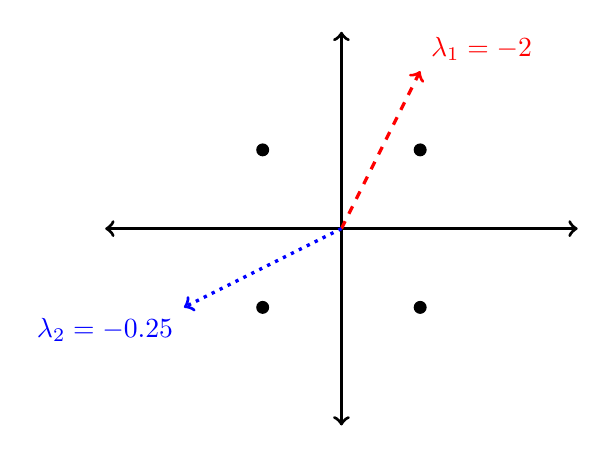
\begin{tikzpicture}
            \draw[very thick, <->, black] (-3,0) -- (3,0);
            \draw[very thick, <->, black] (0,-2.5) -- (0,2.5);
            \draw[very thick, red, ->, dashed] (0,0) -- (1,2) node[anchor=south
            west]{$\lambda_1 = -2$}; 
            \draw[very thick, blue, ->, dotted] (0,0) -- (-2,-1) node[anchor=north
            east]{$\lambda_2 = -0.25$}; 
            \draw[fill=black] (1.0,1.0) circle(0.075cm);
            \draw[fill=black] (-1,-1) circle(0.075cm);
            \draw[fill=black] (-1,1) circle(0.075cm);
            \draw[fill=black] (1,-1) circle(0.075cm);
        \end{tikzpicture}\hspace{0.4in}
        \begin{tikzpicture}
            \draw[very thick, <->, black] (-3,0) -- (3,0);
            \draw[very thick, <->, black] (0,-2.5) -- (0,2.5);
            \draw[very thick, red, ->, dashed] (0,0) -- (1,2) node[anchor=south
            west]{$\lambda_1 = 2$}; 
            \draw[very thick, blue, ->, dotted] (0,0) -- (-2,-1) node[anchor=north
            east]{$\lambda_2 = -0.25$}; 
            \draw[fill=black] (1.0,1.0) circle(0.075cm);
            \draw[fill=black] (-1,-1) circle(0.075cm);
            \draw[fill=black] (-1,1) circle(0.075cm);
            \draw[fill=black] (1,-1) circle(0.075cm);
        \end{tikzpicture}
    \end{center}
    \begin{center}
        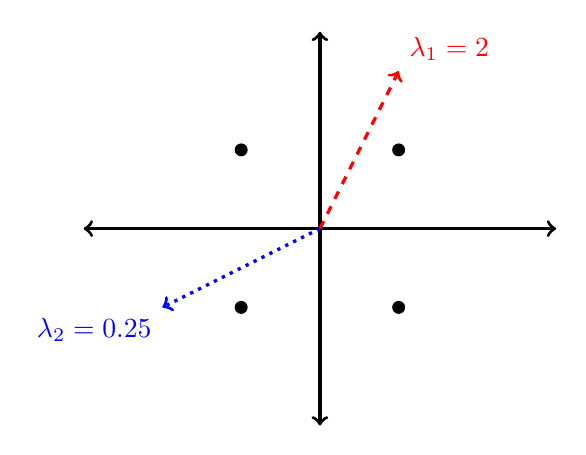
\begin{tikzpicture}
            \draw[very thick, <->, black] (-3,0) -- (3,0);
            \draw[very thick, <->, black] (0,-2.5) -- (0,2.5);
            \draw[very thick, red, ->, dashed] (0,0) -- (1,2) node[anchor=south
            west]{$\lambda_1 = 2$}; 
            \draw[very thick, blue, ->, dotted] (0,0) -- (-2,-1) node[anchor=north
            east]{$\lambda_2 = 0.25$}; 
            \draw[fill=black] (1.0,1.0) circle(0.075cm);
            \draw[fill=black] (-1,-1) circle(0.075cm);
            \draw[fill=black] (-1,1) circle(0.075cm);
            \draw[fill=black] (1,-1) circle(0.075cm);
        \end{tikzpicture}\hspace{0.4in}
        \begin{tikzpicture}
            \draw[very thick, <->, black] (-3,0) -- (3,0);
            \draw[very thick, <->, black] (0,-2.5) -- (0,2.5);
            \draw[very thick, red, ->, dashed] (0,0) -- (1,2) node[anchor=south
            west]{$\lambda_1 = -2+i$}; 
            \draw[very thick, blue, ->, dotted] (0,0) -- (-2,-1) node[anchor=north
            east]{$\lambda_2 = -2-i$}; 
            \draw[fill=black] (1.0,1.0) circle(0.075cm);
            \draw[fill=black] (-1,-1) circle(0.075cm);
            \draw[fill=black] (-1,1) circle(0.075cm);
            \draw[fill=black] (1,-1) circle(0.075cm);
        \end{tikzpicture}
    \end{center}
    \begin{center}
        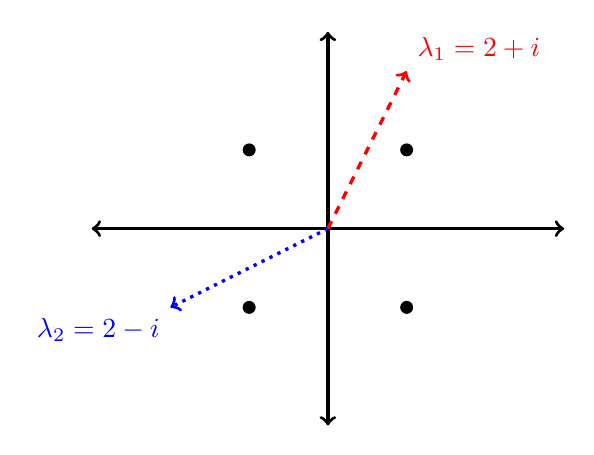
\begin{tikzpicture}
            \draw[very thick, <->, black] (-3,0) -- (3,0);
            \draw[very thick, <->, black] (0,-2.5) -- (0,2.5);
            \draw[very thick, red, ->, dashed] (0,0) -- (1,2) node[anchor=south
            west]{$\lambda_1 = 2+i$}; 
            \draw[very thick, blue, ->, dotted] (0,0) -- (-2,-1) node[anchor=north
            east]{$\lambda_2 = 2-i$}; 
            \draw[fill=black] (1.0,1.0) circle(0.075cm);
            \draw[fill=black] (-1,-1) circle(0.075cm);
            \draw[fill=black] (-1,1) circle(0.075cm);
            \draw[fill=black] (1,-1) circle(0.075cm);
        \end{tikzpicture}\hspace{0.4in}
        \begin{tikzpicture}
            \draw[very thick, <->, black] (-3,0) -- (3,0);
            \draw[very thick, <->, black] (0,-2.5) -- (0,2.5);
            \draw[very thick, red, ->, dashed] (0,0) -- (1,2) node[anchor=south
            west]{$\lambda_1 = i$}; 
            \draw[very thick, blue, ->, dotted] (0,0) -- (-2,-1) node[anchor=north
            east]{$\lambda_2 = -i$}; 
            \draw[fill=black] (1.0,1.0) circle(0.075cm);
            \draw[fill=black] (-1,-1) circle(0.075cm);
            \draw[fill=black] (-1,1) circle(0.075cm);
            \draw[fill=black] (1,-1) circle(0.075cm);
        \end{tikzpicture}
    \end{center}
\end{problem}

Now that we know the general behavior of all $2 \times 2$ systems based on the
eigen-structure let's get a faster way to make the determination.  That is, if we can
avoid actually finding the eigenvalues that might save some time.
\begin{problem}
    Let the $2 \times 2$ linear system $\bx' = A \bx$ be written as
    \[ \begin{pmatrix} x' \\ y' \end{pmatrix} = \begin{pmatrix} a & b \\ c & d
        \end{pmatrix} \begin{pmatrix} x \\ y \end{pmatrix} \]
    Your Tasks:
    \begin{enumerate}
        \item What is the equilibrium of this system presuming that $A^{-1}$ exists?
        \item Find the characteristic polynomial of the coefficient matrix
        \item Simplify the characteristic polynomial to fill in the blanks:
            \[ \lambda^2 + \underline{\hspace{0.5in}} \lambda + \underline{\hspace{0.5in}}
                = 0
                \]
            The blanks should be familiar features of the matrix.
    \end{enumerate}
\end{problem}
\solution{
    The solution to the system is $\bx = \bo$ since we solve $\bo = A
    \bx$ to find the equilibrium and if $A^{-1}$ exists then $\bx = \bo$.  

    The characteristic polynomial is:
$p(\lambda) = \lambda^2 - tr(A) \lambda + \det(A) $
}



\begin{problem}
    In the previous problems you found that the characteristic polynomial for a 2D linear
    system is $p(\lambda) = \lambda^2 - T \lambda + D$ where $T = \text{tr}(A)$ and $D=
    \det(A)$.  Solving for $\lambda$ we see that
    \[ \lambda = \frac{T \pm \sqrt{T^2 - 4 D}}{2}. \]
    Clearly the behavior of the eigenvalues depends on the quantity $T^2 - 4D$.  To
    visualize this we create the {\it trace-determinant} plane as seen in the figure
    immediately below.  Fill in the question marks in the figure with the type of behavior
    you expect to see for each region of the {\it trace-determinant} plane?

    To illustrate what we mean condsider the furthest right question mark.  In that
    question mark the determinant, $D$, is greater than zero, the trace, $T$, is greater
    than zero and $D < T^2 / 4$.  Hence $T^2 - 4D>0$ so we expect the behavior of the
    system to be a nodal source since both eigenvalues will be real and positive.

    Use the following words to fill in the question marks: nodal source, nodal sink,
    spiral source, spiral sink, center, and saddle.
\end{problem}
    \vspace{-0.1in}
        \begin{center}
            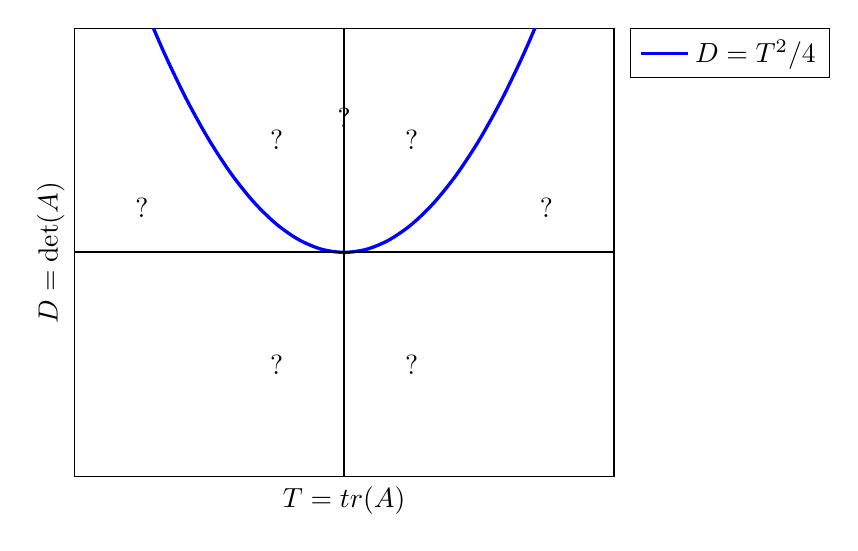
\begin{tikzpicture}
                \begin{axis}[xlabel={$T=tr(A)$},ylabel={$D=\det(A)$}, ymin=-0.5,
                        ymax=0.5, xmin=-2, xmax=2, xtick=\empty, ytick=\empty, legend pos=outer
                    north east]
                    \addplot[smooth,blue, very thick, domain=-2:2] {(1/4)*x^2};
                    \addlegendentry{$D = T^2/4$};
                    \addplot[smooth, black, thick] {0*x};
                    \draw[black,thick] (axis cs:0,-0.5) -- (axis cs:0,0.5);
                    \node at (axis cs:1.5,0.1) {?};
                    \node at (axis cs:-1.5,0.1) {?};
                    \node at (axis cs:-.5,0.25) {?};
                    \node at (axis cs:.5,0.25) {?};
                    \node at (axis cs:0,0.3) {?};
                    \node at (axis cs:0.5,-0.25) {?};
                    \node at (axis cs:-0.5,-0.25) {?};
                \end{axis}
            \end{tikzpicture}
        \end{center}

\solution{
        \begin{center}
            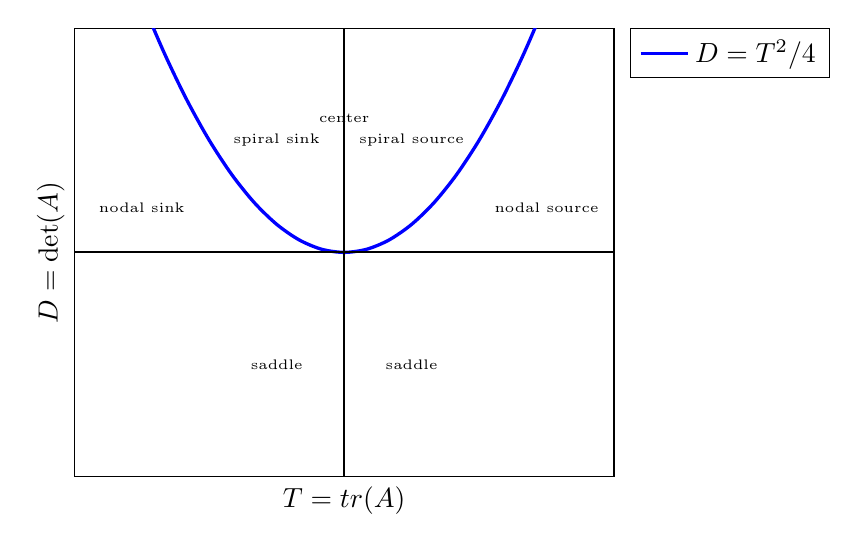
\begin{tikzpicture}
                \begin{axis}[xlabel={$T=tr(A)$},ylabel={$D=\det(A)$}, ymin=-0.5,
                        ymax=0.5, xmin=-2, xmax=2, xtick=\empty, ytick=\empty, legend pos=outer
                    north east]
                    \addplot[smooth,blue, very thick, domain=-2:2] {(1/4)*x^2};
                    \addlegendentry{$D = T^2/4$};
                    \addplot[smooth, black, thick] {0*x};
                    \draw[black,thick] (axis cs:0,-0.5) -- (axis cs:0,0.5);
                    \node at (axis cs:1.5,0.1) {\tiny{nodal source}};
                    \node at (axis cs:-1.5,0.1) {\tiny{nodal sink}};
                    \node at (axis cs:-.5,0.25) {\tiny{spiral sink}};
                    \node at (axis cs:.5,0.25) {\tiny{spiral source}};
                    \node at (axis cs:0,0.3) {\tiny{center}};
                    \node at (axis cs:0.5,-0.25) {\tiny{saddle}};
                    \node at (axis cs:-0.5,-0.25) {\tiny{saddle}};
                \end{axis}
            \end{tikzpicture}
        \end{center}
    }

% \begin{problem}
%     Modeling a bungee jumper is much like modeling a 1-dimensional spring mass system
%     except for the fact that
%     the air resistance plays a major role.  According to Newton's second law as well as
%     Hooke's law
%     \[ m x'' = -kx + F_{drag} \quad \text{where} \quad F_{drag} = -a x' \]
%     Hence, the model for the motion of the bungee jumper is
%     \[ mx'' + ax' + kx = 0 \]
%     Dividing by mass we get
%     \[ x'' + \alpha x' + \kappa x = 0 \]
%     Turn this into a system of differential equations with an appropriate substitution,
%     discuss equilibria and stability, and explore it graphically.
% \end{problem}
% \solution{This is a straight foward linear system
%     \[ \left\{ \begin{array}{ll} x' &= y \\ y' &= - \alpha y - \kappa x \end{array}
%     \right. \]
%     Equlibrium: $(0,0)$.  Stable.
%     \[ A = \begin{pmatrix} 1 & 0 \\ -\kappa & -\alpha \end{pmatrix} \]
%     so 
%     \[ \lambda_{1,2} = \frac{-\alpha \pm \sqrt{\alpha^2 - 4 \kappa}}{2} \]
%     The real part is negative so the equilibrium is stable.
% 
% }

Now we'll finally look at some nonlinear systems.
\begin{problem}\label{prob:competin_species}
    Suppose that $x$ and $y$ are the population of two distinct species that compete for the
    same resources. For example, two species of fish may compete for the same food in a
    lake or sheep and cattle competing for the same grazing land. We can model two
    competing species using the following system of first-order differential equations, 
    \begin{flalign*}
        x' &= 2x\left( 1-\frac{x}{2} \right) - xy \\
        y' &= 3y\left( 1-\frac{y}{3} \right) - 2xy.
    \end{flalign*}
    It is reasonably easy to show that the four equilibrium solutions are $(0,0)$,
    $(0,3)$, $(2,0)$, and $(1,1)$.  Use the \texttt{pplane} software (linked from Moodle)
    to analyze what happens near the equilibrium $(1,1)$.
\end{problem}


Now we'll build up the analytic tools necessary to analyze the competing species model in
problem \ref{prob:competin_species}.
\begin{definition}[Nullclines and Equilibria]
    The {\bf nullclines} for a linear system 
    \begin{flalign*}
        x'(t) &= f(x,y) \\
        y'(t) &= g(x,y)
    \end{flalign*}
    are the curves where $f(x,y)=0$ and $g(x,y)=0$.  When two nullclines intersect there
    is and equilibrium solution.
\end{definition}
\begin{problem}
    Use a graphing tool to sketch the nullclines of the system and use your graph to
    verify the location of the equilibrium points.
    \begin{flalign*}
        x' &= 2x\left( 1-\frac{x}{2} \right) - xy \\
        y' &= 3y\left( 1-\frac{y}{3} \right) - 2xy.
    \end{flalign*}
\end{problem}
\solution{
    The nullclines are $2x(1-x/2)-xy=0$ and $3y(1-y/3)-2xy = 0$.  In the first one we
    either have the vertical line $x=0$ or the line $y=2(1-x/2)$.  In the second one we
    either have the horizontal line $y=0$ of the line $2x = 3(1-y/3)$.  Plotting all four
    of these lines together we see that the intersections are $(0,0)$, $(0,3)$, $(2,0)$,
    and $(1,1)$.
}

\begin{definition}[Jacobian Matrix]
    Consider the system of equations
    \begin{flalign*}
        f(x,y) &= 0 \\
        g(x,y) &= 0.
    \end{flalign*}
    The {\bf Jacobian matrix} for this system is defined as
    \[ J(x,y) = \begin{pmatrix} f_x & f_y \\ g_x & g_y \end{pmatrix} \]
    where subscripts mean partial dervatives.
\end{definition}

\begin{problem}
    Find the Jacobian matrix $J(x,y)$ for the system 
    \begin{flalign*}
        x' &= 2x\left( 1-\frac{x}{2} \right) - xy = 2x - x^2 - xy \\
        y' &= 3y\left( 1-\frac{y}{3} \right) - 2xy = 3y - y^2 - 2xy.
    \end{flalign*}
\end{problem}
\solution{
    \[ J(x,y) = \begin{pmatrix} 2-2x-y & -x \\ -2y & 3-2y-2x \end{pmatrix} \]
}

The Jacobian describes the local linear behavior of the system near an equilibrium.  That
is to say that if we substitute the values $(x_*,y_*)$ from an equilibrium point into the Jacobian
then {\it near} the equilibrium point will behave like the linear system $\bx' =
J(x_*,y_*) \bx$ centered at the equilibrium.  

\begin{problem}
    Verify the behavior of the system 
    \begin{flalign*}
        x' &= 2x\left( 1-\frac{x}{2} \right) - xy \\
        y' &= 3y\left( 1-\frac{y}{3} \right) - 2xy
    \end{flalign*}
    near the equilibrium $(1,1)$ (you already discussed this in Problem
    \ref{prob:competin_species}).  Then use the Jacobian matrix to discuss the behavior of
    the system near the other three equilibria.
\end{problem}
\solution{
    At $(1,1)$ we have $J(1,1) = \begin{pmatrix} -1 & -1 \\ -2 & -1 \end{pmatrix}$.
        Observe that $\text{tr}(J(1,1)) = -2$ and $\det(J(1,1)) = 1 - 2 = -1$.  From the
        trace-determinant plane we should have a saddle near $(1,1)$.
}



\begin{technique}[Equilibria and Stability of Nonlinear Systems]
    Consider the nonlinear system of differential equations
    \begin{flalign*}
        x'(t) &= f(x,y) \\
        y'(t) &= g(x,y).
    \end{flalign*}
    To find and analyze the equilibria for the system:
    \begin{enumerate}
        \item Find the equilibria by setting \underline{\hspace{0.5in}} to zero and
            solving for $x$ and $y$.  It may be necessary to use technology to solve this
            system of nonlinear equations.
        \item Find the Jacobian matrix at each of the equilibrium points.
        \item Investigate the \underline{\hspace{0.5in}} for each Jacobian matrix.  Based
            on this investigate you can make a claim about local stability.
    \end{enumerate}
\end{technique}

\begin{example}
    Consider the system 
    \begin{flalign*}
        x'(t) &= x-3y+xy^2 \\
        y'(t) &=  2x-4y-x^2y.
    \end{flalign*}
    Find the nullclines, equilibria, the Jacobian, and classify the equilibrium solutions.
    \\ {\bf Solution:} \\
    The nullclines are the curves $f(x,y) = 0$ and $g(x,y) = 0$ called the $x$-nullcline
    and the $y$-nullcline respectively since if $f=0$ the $x$-variable stops changing and
    if $g=0$ the $y$-variable stops changing.  
    \begin{flalign*}
        \text{$x$-nullcline: } 0&= x-3y+xy^2\\
        \text{$y$-nullcline: } 0&= 2x - 4y - x^2y
    \end{flalign*}
    These are rather complicated curves in the $xy$-plane.

    Using a computer algebra system the approximate equilibria are $(-1.06, -0.41)$, $(1.06,
    0.41)$, and $(0,0)$ (along with a few imaginary equilibria).

    The Jacobian is $J(x,y) = \begin{pmatrix} 1+y^2 & -3 + 2xy \\ 2-2xy & -4-x^2
    \end{pmatrix}$ 
    and at $(0,0)$ we have $J(0,0) = \begin{pmatrix} 1 & -3 \\ 2 & -4 \end{pmatrix}$.  For
    this equilibrium point, $T(0,0) = -3$ and $D(0,0) = (-4) - (-6) = 2$.  Hence $T^2/4 =
    9/4 = 2.25 > D$ so according to the trace-determinant plane we much have a spiral
    sink at $(0,0)$.
\end{example}




\newpage\section{Applied Nonlinear Systems}
Let's get started with a nonlinear system.  This system will be familiar in a lot of ways
but we will added a small wrinkle: air resistance.





\begin{problem}
    Modeling a bungee jumper is much like modeling a 1-dimensional spring mass system
    except for the fact that
    the air resistance plays a major role.  According to Newton's second law as well as
    Hooke's law
    \[ m x'' = -kx + F_d \quad \text{where} \quad F_d = -a x' -b \left( x' \right)^2 \]
    Hence, the model for the motion of the bungee jumper is
    \[ mx'' + ax' + b\left( x' \right)^2 + ky = 0 \]
    Dividing by mass we get
    \[ x'' + \alpha x' + \beta \left( x' \right)^2 + \kappa x = 0 \]
    Turn this into a system of differential equations with an appropriate substitution,
    discuss equilibria and stability, and explore it graphically.
\end{problem}
\solution{
    Let $x'=y$ and get the following:
    \[ \left\{ \begin{array}{ll} x'&= y \\ y' &= -\alpha y - \beta y^2 - \kappa x
    \end{array} \right. \]
    This is a nonlinear system!!

    Equlibria: Set $x'=y'=0$
    \[ \left\{ \begin{array}{ll} 0&= y \\ 0 &= -\alpha y - \beta y^2 - \kappa x
    \end{array} \right. \]
    Therefore, $x=y=0$ is the equilibrium.

    Local stability: Find the Jacobian:
    \[ J(x,y) = \begin{pmatrix} f_x & f_y \\ g_x & g_y \end{pmatrix} = \begin{pmatrix} 0 &
        1 \\ -\kappa & -\alpha - 2\beta y \end{pmatrix} \]
    \[ \implies J(0,0) = \begin{pmatrix} 0 & 1 \\ -\kappa & -\alpha \end{pmatrix} \]
    and we are locally back at the same spot as the linear problem. Hence the equilibrium
    is locally stable.
}


\begin{problem}
    Suppose that we have a predator-prey system consisting of a population of foxes ($F$)
    and rabbits ($R$)
    \begin{flalign*}
        R'(t) &= 2R - RF \\
        F'(t) &= -5F + RF.
    \end{flalign*}
    It is easy to check that have equilibrium at $R=5$ and $F=2$.  Fully analyze the
    dynamics of the population assuming that it doesn't start with $(R,F) = (5,2)$.  In
    particular, make a phase plot and determine the stability of the equilibrium.
\end{problem}
\solution{(Modified from \cite{Judson}) 
}

\begin{problem}
    In the previous problem, modify the rabbit population so that it follows logistic
    growth
    \[ R'(t) = 2R\left( 1-\frac{R}{10} \right) - RF. \]
    Fully analyze this new system.
\end{problem}
\solution{spiral sink at $(5,1)$}

\begin{problem}
    Romeo and Juliet's love can be quantified as
    \begin{center}
        \begin{tabular}{|c|c|}
            \hline
            Hysterical Hatred & $-5$ \\
            Disgust & $-2.5$ \\
            Indifference & $0$ \\
            Sweet Affection & $2.5$ \\
            Ecstatic Love & $5$ \\ \hline
        \end{tabular}
    \end{center}
    The characters struggle with frustrated love due to the lack of reciprocity of their
    feelings.
    \begin{description}
        \item[Romeo:] ``My feelings for Juliet decrease in proportion to her love for
            me.''
        \item[Juliet:] ``My love for Romeo grows in proportion to his love for me.''
    \end{description}
    Write a mathematical model for the ill-fated love of Romeo and Juliet.  Discuss
    equilibria and stability. Explore graphically. \\Assume $R(0) = 2$ and $J(0)=0$.  What do these initial
    conditions mean? Start your explorations with $\alpha = 0.2$ and $\beta = 0.8$.
\end{problem}
\solution{
    \[ \left\{ \begin{array}{ll} R' &= -\alpha J \\ J' &= \beta R \end{array} \right. \]
    Linear, so
    \[ \begin{pmatrix} 0 & -\alpha \\ \beta & 0 \end{pmatrix} \]
    \[ \implies \lambda_{1,2} = \pm \sqrt{-\alpha \beta} \]
    so there will be oscillations so long as $\alpha,\beta > 0$.

    Take $\alpha = 0.2$ and $\beta = 0.8$ for an interesting exploration.
}



\begin{problem}
    Romeo and Juliet's love can be quantified as
    \begin{center}
        \begin{tabular}{|c|c|}
            \hline
            Hysterical Hatred & $-5$ \\
            Disgust & $-2.5$ \\
            Indifference & $0$ \\
            Sweet Affection & $2.5$ \\
            Ecstatic Love & $5$ \\ \hline
        \end{tabular}
    \end{center}
    The characters struggle with frustrated love due to the lack of reciprocity of their
    feelings.
    \begin{description}
        \item[Romeo:] ``My feelings for Juliet decrease in proportion to her love for
            me.''
        \item[Juliet:] ``My love for Romeo grows in proportion to his love for me.''
            But, her emotional swings lead to sleepless nights which consequently
            dampen her emotions.
    \end{description}
    Write a mathematical model for the ill-fated love of Romeo and Juliet.  Discuss
    equilibria and stability. Explore graphically. 
\end{problem}
\solution{
    \[ \left\{ \begin{array}{ll} R' &= -\alpha J \\ J' &= \beta R - \kappa J^r\end{array} \right. \]
    If $r=1$ then this is linear, so
    \[ \begin{pmatrix} 0 & -\alpha \\ \beta & \kappa \end{pmatrix} \]
    \[ \implies \lambda_{1,2} = \frac{-\kappa \pm \sqrt{\kappa^2 - 4 \alpha \beta }}{2} \]
    So there could be oscillations but since the real part is negative there will be an
    overall damping and the end result will be a stable equilibrium at $(R,J) = (0,0)$.

    If $r \ne 1$ then:\\
    \[ J(x,y) = \begin{pmatrix} 0 & -\alpha \\ \beta & r \kappa J^{r-1} \end{pmatrix} \]
    You will still have the same local stability.

}


\begin{problem}
    In historical battles where hand-to-hand combat was common, a mathematical model
    for the survival of the various forces is:
    \begin{itemize}
        \item The rate at which the {\color{red} RED} army loses troops is
            proportional to the product of the sizes of the two armies
        \item The rate at which the {\color{blue} BLUE} army loses troops is
            proportional to the product of the sizes of the two armies
    \end{itemize}
    Write a mathematical model for the size of each army.  Discuss equilibria, stability,
    and explore graphically. What is wrong with this model?
\end{problem}
\solution{
    \[ \left\{ \begin{array}{ll} R' &= -\alpha RB \\ B' &= -\beta RB \end{array} \right.
    \]
    Clearly if either $R=0$ OR if $B=0$ then there is an equilibrium.
    \[ J(R,B) = \begin{pmatrix} -\alpha B & -\alpha R \\ -\beta B & \beta R \end{pmatrix}
    \]
    If $R=0$ then $J(0,B) = \begin{pmatrix} -\alpha B & 0 \\ -\beta B & 0 \end{pmatrix}$
    and locally
    \[ \begin{pmatrix} R \\ B \end{pmatrix} = c_1 \begin{pmatrix} 0\\1\end{pmatrix} + c_2
    e^{-\beta t} \begin{pmatrix}1\\1\end{pmatrix} \]
    and any of the equilibrium points will be stable.  Similar for $B=0$.
}

\begin{problem}
    In historical battles where hand-to-hand combat was common, a mathematical model
    for the survival of the various forces is:
    \begin{itemize}
        \item The rate at which the {\color{red} RED} army loses troops is
            proportional to the product of the sizes of the two armies
        \item The rate at which the {\color{blue} BLUE} army loses troops is
            proportional to the product of the sizes of the two armies
        \item The rate at which the {\color{red} RED} army gains recruits is
            proportional to the size of the {\color{red} RED} army.
    \end{itemize}
    Write a mathematical model for the size of each army.  Discuss equilibria, stability,
    and explore graphically. How do you prove stability?
\end{problem}
    \solution{
        \[ \left\{ \begin{array}{ll} R' &= -\alpha RB + \kappa R \\ B' &= -\beta RB \end{array} \right. \]

    }



\newpage\section{Additional Exercises}

\begin{problem}
    The Van der Pol oscillator equation arose in the 1920's when Balthasar Van der Pol was
    working with oscillator circuits for radios.  The equation is
    \[ x'' + \mu (x^2-1) x' + x = 0 \]
    where $x$ is related to the current in an RLC-circuit.  Write the Van der Pol equation
    as a non-linear first order system and completely investigate the behaviour of the system using
    $\mu = 1$.  Use \texttt{pplane} plots to aid in your analysis.
\end{problem}
\solution{
The first order nonlinear system is
\begin{flalign*}
    x'(t) &= y \\
    y'(t) &= -x - \mu(x^2-1)y
\end{flalign*}
The only equilibrium point is $(x,y) = (0,0)$ and the Jacobian is
\[ J(x,y)  \begin{pmatrix} 0 & 1 \\ -1-2\mu x y & -\mu(x^2-1) \end{pmatrix} \]
so at $(0,0)$ we have
\[ J(0,0) = \begin{pmatrix} 0 & 1 \\ -1 & \mu \end{pmatrix}. \]
Since the trace is $\mu$ and the determinant is 1 we know that the origin is a spiral
source.
}

\begin{problem}
    A virus spreads through a dorm.  Assume that there are three types of people in the
    dormitory population: $S$ is the number of people susceptible to the virus, $I$ is the
    number of infectious people, and $R$ is the number of recovered people.  Assume that
    $S+I+R=N$ is the total number of people in the dorm (and $N$ is fixed).  Build a
    differential equation model for the rates at which $S$, $I$, and $R$ change assuming
    that
    \begin{itemize}
        \item The susceptible people get sick at a rate proportional to the interactions
            with infectious people.
        \item Infectious people recover at a fixed rate.
    \end{itemize}
    Once you have your model explore it graphically (using \texttt{pplane}) and analyze
    any equilibrium points. (Hint: you really only need 2 equations)
\end{problem}


\begin{problem}
    The {\bf Western Grasslands Model}: This is a model of the competition between
    ``good'' grass and weeds on a fixed area of rangeland where cattle are
    allowed to graze.  The two dependent variables $g(t)$ and $w(t)$ represent,
    respectively, the fraction of the area colonized by the good grass and the
    weeds at time $t$. Hence, $0 \le g
    \le 1$ and $0 \le w \le 1\}$.  The model is given by
    \begin{flalign*}
        \frac{dg}{dt} &= R_1 g \left(  1 - g - 0.6 w \frac{E + g}{0.31 E + g} \right) \\
        \frac{dw}{dt} &= R_2 g \left(  1 - w - 1.07 g \frac{0.31E + g}{E + g} \right).
    \end{flalign*}
    The parameters $R_1$ and $R_2$ represent the intrinsic growth rates of the grass and
    weeds respectively.  The cattle stocking rate is introduced through the parameter $E$.
    For this problem assume that $R_1 = 0.27$, $R_2 = 0.4$, and $E = 0.3$.  There are
    several equilibrium points that we need to analyze.
    \begin{itemize}
        \item There is an equilibrium at $(0,0)$.  What does it mean physically and what
            type of behavior do we see near this point?
        \item There is an equilibrium at $(0,1)$.  What does it mean physically and what
            type of behavior do we see near this point?
        \item There are two equilibria inside the domain where both weeds and grass can
            coexist.  Find them and describe the behavior of the system near them.
    \end{itemize}
\end{problem}

